\section{Scale-up Server Scalalbility}


\begin{figure*}[tb]
    \centering
    \begin{subfigure}[b]{0.25\textwidth}
        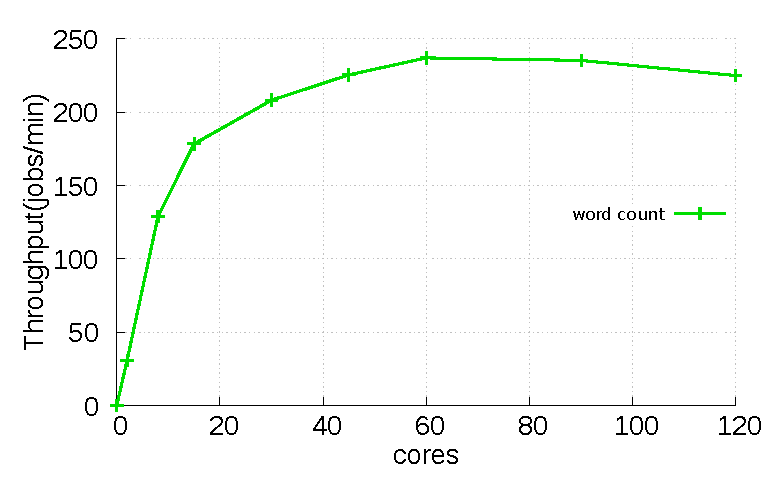
\includegraphics[width=1.8in]{graph/wc.eps}
        \caption{Word Count}
    \end{subfigure}%
    \begin{subfigure}[b]{0.25\textwidth}
        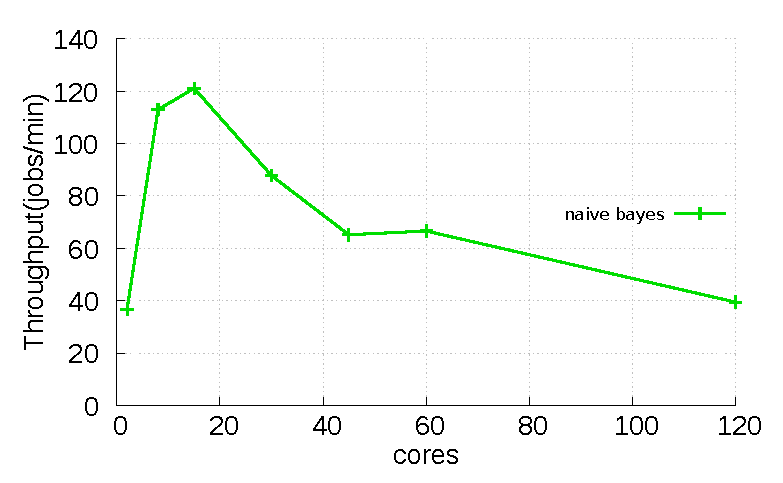
\includegraphics[width=1.8in]{graph/nb.eps}
        \caption{Naive Basian}
    \end{subfigure}%
    \begin{subfigure}[b]{0.25\textwidth}
        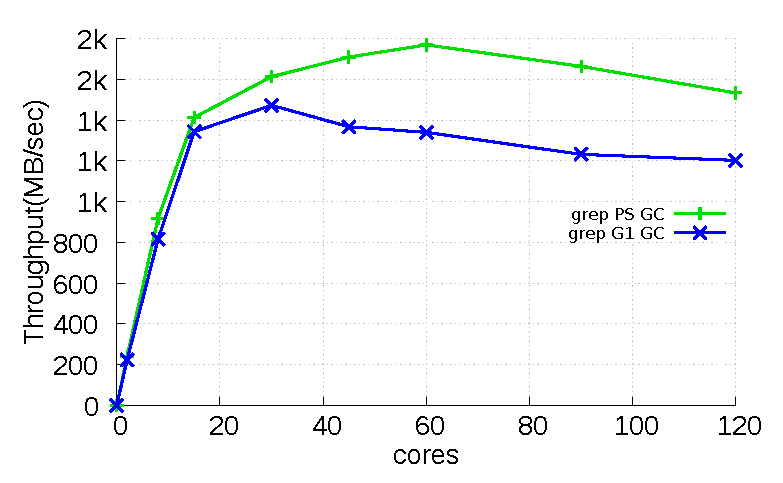
\includegraphics[width=1.8in]{graph/grep.eps}
        \caption{Grep}
    \end{subfigure}%
    \begin{subfigure}[b]{0.25\textwidth}
        \includegraphics[width=1.8in]{graph/kmeans.eps}
        \caption{K-means}
    \end{subfigure}%
    \caption{CPU utilization on 120 core.}
    \label{fig:utilization}
\end{figure*}



\begin{figure*}[tb]
    \centering
    \begin{subfigure}[b]{0.25\textwidth}
        \includegraphics[width=1.8in]{graph/wc_cpuutils.eps}
        \caption{Word Count}
    \end{subfigure}%
    \begin{subfigure}[b]{0.25\textwidth}
        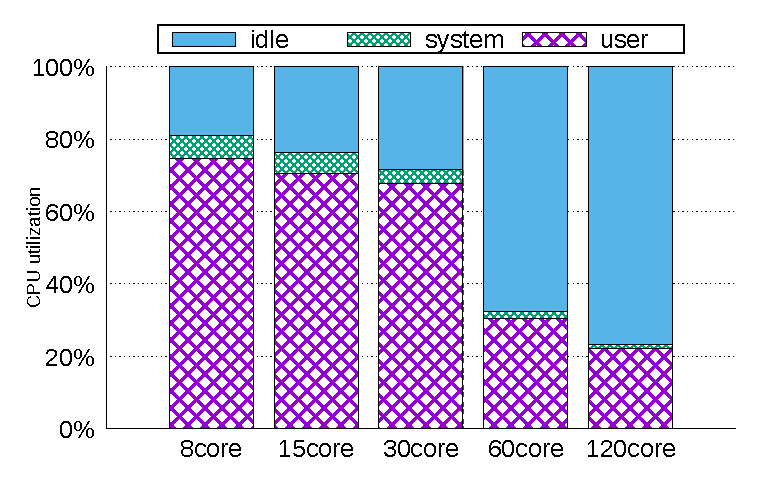
\includegraphics[width=1.8in]{graph/nb_cpuutils.eps}
        \caption{Naive Basian}
    \end{subfigure}%
    \begin{subfigure}[b]{0.25\textwidth}
        \includegraphics[width=1.8in]{graph/grep_cpuutils.eps}
        \caption{Grep}
    \end{subfigure}%
    \begin{subfigure}[b]{0.25\textwidth}
        \includegraphics[width=1.8in]{graph/kmeans_cpuutils.eps}
        \caption{K-means}
    \end{subfigure}%
        \centering
    \caption{CPU utilization on 120 core.}
    \label{fig:utilization}
\end{figure*}
Figure~\ref{fig:utilization}(a)) since it waits to acquire



%$$$$$$$$$$$$$$$$$$$$$$$$$$$$$$$$$$$$$$$$$$$$$$$$$$$$$$$$$$$$$$$$$$$$$$$$$$$$$$$$
%$$$$$$$$$$$$$$$$$$$$$$$$$$$$$$$$$$$$$$$$$$$$$$$$$$$$$$$$$$$$$$$$$$$$$$$$$$$$$$$$
% 이번 장에 대한 설명
%$$$$$$$$$$$$$$$$$$$$$$$$$$$$$$$$$$$$$$$$$$$$$$$$$$$$$$$$$$$$$$$$$$$$$$$$$$$$$$$$
\ifkor
본 장에서는 single node로 구성된 scale-up 서버에서의 spark scalability에
분석한 내용에 대해 설명한다. 
\else

\fi



\subsection{Test-bed and Benchmark}

%$$$$$$$$$$$$$$$$$$$$$$$$$$$$$$$$$$$$$$$$$$$$$$$$$$$$$$$$$$$$$$$$$$$$$$$$$$$$$$$$
%$$$$$$$$$$$$$$$$$$$$$$$$$$$$$$$$$$$$$$$$$$$$$$$$$$$$$$$$$$$$$$$$$$$$$$$$$$$$$$$$
% Apache Spark에 대한 설명
%$$$$$$$$$$$$$$$$$$$$$$$$$$$$$$$$$$$$$$$$$$$$$$$$$$$$$$$$$$$$$$$$$$$$$$$$$$$$$$$$
\ifkor
\noindent
\textbf{Apache Spark. }
Apache Spark is open-source data analytics frameworks, designed to operate on
datasets larger than can be process on a single node while automatically
providing for scheduling and load-balancing.
\else

\fi

%$$$$$$$$$$$$$$$$$$$$$$$$$$$$$$$$$$$$$$$$$$$$$$$$$$$$$$$$$$$$$$$$$$$$$$$$$$$$$$$$
%$$$$$$$$$$$$$$$$$$$$$$$$$$$$$$$$$$$$$$$$$$$$$$$$$$$$$$$$$$$$$$$$$$$$$$$$$$$$$$$$
% 테스트 베드 설명
%$$$$$$$$$$$$$$$$$$$$$$$$$$$$$$$$$$$$$$$$$$$$$$$$$$$$$$$$$$$$$$$$$$$$$$$$$$$$$$$$
\ifkor
\noindent
\textbf{Test-bed. }
Our Intel platform is composed of Xeon E5 Each CPU exploits the Iby Brige
technoloy and consists in a multi-core architecture.
We use two machines to evaluate conflict-free and conflicting operations on real hardware: an
80-core (8 sockets × 10 cores) Intel Xeon E7-8870 (the same machine used for evaluation in
chapter 9) and, to show that our conclusions generalize, a 48-core (8 sockets × 6 cores) AMD
the two manufacturers use different architectures, interconnects, and coherence protocols.

\begin{figure}[h]
  \begin{center}
     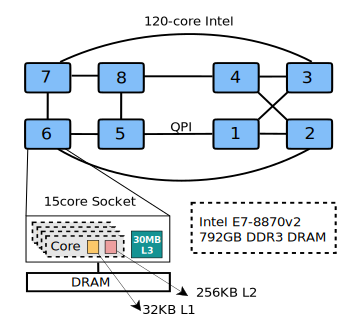
\includegraphics[width=0.4\textwidth]{fig/xeon}
  \end{center}
  \caption{test-bed intel xeon archtecture.}
  \label{fig:basic}
\end{figure}
Hyper-Threading is disabled, and Linux kernel 4.5-rc6.
\else

\fi

%$$$$$$$$$$$$$$$$$$$$$$$$$$$$$$$$$$$$$$$$$$$$$$$$$$$$$$$$$$$$$$$$$$$$$$$$$$$$$$$$
%$$$$$$$$$$$$$$$$$$$$$$$$$$$$$$$$$$$$$$$$$$$$$$$$$$$$$$$$$$$$$$$$$$$$$$$$$$$$$$$$
%Benchamrk에 대한 설명
%$$$$$$$$$$$$$$$$$$$$$$$$$$$$$$$$$$$$$$$$$$$$$$$$$$$$$$$$$$$$$$$$$$$$$$$$$$$$$$$$
\ifkor
\noindent
\textbf{Benchmark.} 벤치마크와 워크로드에 대한 BigData Benchmark를 사용하였다.
\begin{itemize}
\item \textbf{Word Count. }We have developed a novel lightweight log-based
structures with efficient log management implementation.
\item \textbf{Grep. }
We applied the in Linux kernel to two reverse mapping(anonymous, file) on
Our design improved throughput and execution time from 1.5x through 2.7x on 120 core.
\item \textbf{Naive Basian. }
We applied the in Linux kernel to two reverse mapping(anonymous, file) on
Our design improved throughput and execution time from 1.5x through 2.7x on 120 core.
\item \textbf{K-means.}
We applied the in Linux kernel to two reverse mapping(anonymous, file) on
Our design improved throughput and execution time from 1.5x through 2.7x on 120 core.
\end{itemize}
\else

\fi


\subsection{Spark Scalability Problem}
%$$$$$$$$$$$$$$$$$$$$$$$$$$$$$$$$$$$$$$$$$$$$$$$$$$$$$$$$$$$$$$$$$$$$$$$$$$$$$$$$
%$$$$$$$$$$$$$$$$$$$$$$$$$$$$$$$$$$$$$$$$$$$$$$$$$$$$$$$$$$$$$$$$$$$$$$$$$$$$$$$$
%Scalability 결과에 대한 대략 적인 설명
%$$$$$$$$$$$$$$$$$$$$$$$$$$$$$$$$$$$$$$$$$$$$$$$$$$$$$$$$$$$$$$$$$$$$$$$$$$$$$$$$
\ifkor
Figure 1 shows the spark scalability of five workload.
실험 결과 60코어까지는, scalability를 가지다가 60코어 이후에는 scalability 문제가 생겼다.
그 이유는 GC에 의해 serialized 되는 부분과 NUMA에 대한 영향 때문에 scalability가 떨어진다.
Word Count와 XXXX XXXX는 비슷한 결과를 가진다.
하지만 Pagerank는 다른 결과를 가지는데 그 이유는 XX
Shared memory 시스템의 공유데이터 때문에 발생하는 scalability 저해 요소 때문에 필요하다.
첫째로 공유 데이터를 lock이 있다. 표 xxx 앞에서 실험한 spark의 wordcount에 대해서 .
\else

\fi

%$$$$$$$$$$$$$$$$$$$$$$$$$$$$$$$$$$$$$$$$$$$$$$$$$$$$$$$$$$$$$$$$$$$$$$$$$$$$$$$$
%$$$$$$$$$$$$$$$$$$$$$$$$$$$$$$$$$$$$$$$$$$$$$$$$$$$$$$$$$$$$$$$$$$$$$$$$$$$$$$$$
%GC 영향에 대한 대략 적인 설명
%$$$$$$$$$$$$$$$$$$$$$$$$$$$$$$$$$$$$$$$$$$$$$$$$$$$$$$$$$$$$$$$$$$$$$$$$$$$$$$$$
\ifkor
우리는 scalable한 GC를 2가지를 대상으로 실험을 해보았다.
실험 결과 GC의 종류에 따른 성능차이는 크다.
먼저 GxXXX GC는 가장 높은 성능을 가졌으며, 다른 GC들은 이것보다는 낮은 성능을
보였다. 
하지만 아무리 Pararall한 GC를 사용한다고 해도 여전히 scalability 문제는 존재한다.
JVM 위에서 동작하는 thread간의 공유하는 single address space때문에 발생하는 공유 문제이다.
다음으로 scheduler가 아직 
\else

\fi




%$$$$$$$$$$$$$$$$$$$$$$$$$$$$$$$$$$$$$$$$$$$$$$$$$$$$$$$$$$$$$$$$$$$$$$$$$$$$$$$$
%$$$$$$$$$$$$$$$$$$$$$$$$$$$$$$$$$$$$$$$$$$$$$$$$$$$$$$$$$$$$$$$$$$$$$$$$$$$$$$$$
%CPU utilization에 대한 설명
%$$$$$$$$$$$$$$$$$$$$$$$$$$$$$$$$$$$$$$$$$$$$$$$$$$$$$$$$$$$$$$$$$$$$$$$$$$$$$$$$

\ifkor
CPU utilization은 그림 XX-XX와 같다. 
node에 동작하는 시스템의 scalability 특성을 고려하지 않았기 때문이다. 
scale-up server를 위한 spark scalability의 근본적인 해결 방법은 spark library와 
runtime엔진을 scale-up서버를 위해 scalable하게 만드는 것이다.
하지만 scale-out 시스템의 scalability를 위해 작성된 spark의 library와 runtime 엔진을 
수정하는것은 쉽지않다.
\else

\fi


%$$$$$$$$$$$$$$$$$$$$$$$$$$$$$$$$$$$$$$$$$$$$$$$$$$$$$$$$$$$$$$$$$$$$$$$$$$$$$$$$
%$$$$$$$$$$$$$$$$$$$$$$$$$$$$$$$$$$$$$$$$$$$$$$$$$$$$$$$$$$$$$$$$$$$$$$$$$$$$$$$$
% Linux kernel scalability (lock, cache cohearnci, scheduler)등등 OS 노이즈에 대한 설명
%$$$$$$$$$$$$$$$$$$$$$$$$$$$$$$$$$$$$$$$$$$$$$$$$$$$$$$$$$$$$$$$$$$$$$$$$$$$$$$$$
\ifkor
%NUMA의 영향 뿐만 아니라, 추가적으로 operating system의 scalability 저해 요소 때문에 
%파티션닝 방법은 필요하다.
%우리는 operation system에서 scalability의 영향을 주는 것을 확인하기 위해 가장먼저
%lock을 조사해보았다.
%첫째로 공유 데이터를 lock이 있다. 표 xxx 앞에서 실험한 spark의 wordcount에 대해서 .
%JVM 위에서 동작하는 thread간의 공유하는 single address space때문에 발생하는 공유 문제이다.
%다음으로 scheduler가 아직 
%마지막으로 cache cohearci traffic이 있다. 
\else

\fi



\subsection{Benefit of Partitioning}
%\subsection{NUMA}

%$$$$$$$$$$$$$$$$$$$$$$$$$$$$$$$$$$$$$$$$$$$$$$$$$$$$$$$$$$$$$$$$$$$$$$$$$$$$$$$$
%$$$$$$$$$$$$$$$$$$$$$$$$$$$$$$$$$$$$$$$$$$$$$$$$$$$$$$$$$$$$$$$$$$$$$$$$$$$$$$$$
%NUMA 영향에 대한 대략 적인 설명
%$$$$$$$$$$$$$$$$$$$$$$$$$$$$$$$$$$$$$$$$$$$$$$$$$$$$$$$$$$$$$$$$$$$$$$$$$$$$$$$$

\ifkor
Spark의 모든 Thread들은 모두 JVM 위에서 동작하기 때문에, Spark는 JVM에 의존적이다.
따라서 우리는 JVM의 파티션닝에 대한 효과를 분석하기 위해, JVM에서 동작하는 응용프로그램의
성능을 가장 잘 practical하게 측정 할 수 있는 벤치마크인 SPECjbb2013 사용하여 사전에 
파티션닝에 대한 효과를 분석을 하였다. 
파티션닝된  실험은 SPECjbb2013 벤치마크의 JVM 수를 소캣의 갯수와 동일하게 설정하였고, 
메모리 용량을 시스템 최대 가용 용량으로 설정하여 실험하였다. 
실험은 다음과 같이 3가지 설정을 하여 수행하였다. 
자동 NUMA 밸런싱 기능을 사용한 방법(multi-auto)과 사용하지 않은 
방법(multi-base) 그리고 그룹을 노드에 최적화한 방법(multi-pin)을 
사용하여 실험하였다.

\else
\fi

\begin{figure}[h]
  \begin{center}
     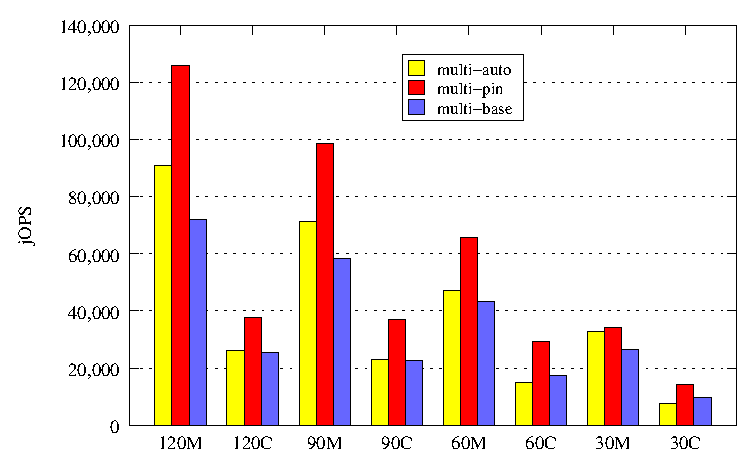
\includegraphics[width=0.4\textwidth]{graph/SPECjbb2013}
  \end{center}
  \caption{Test-bed Intel xeon archtecture.}
  \label{fig:basic}
\end{figure}

\ifkor
실험 결과 대부분 응용프로그램에서 최적화된 파티션으로 설정한 방법이 가장 좋은 
성능을 보였고, 다음으로 자동 NUMA 밸런싱이 좋은 성능을 나타낸다. 
마지막으로 자동 NUMA 밸런싱을 사용하지 않으면 최악의 성능을 보였다.
이것은 아직까지는 리눅스 커널에 autoNUMA의 기술이 향상 되고 있어도, 
잘 파티션되어 동작할 때와 많은 성능 차이를 보여준다[]. 
\else
\fi
